% Copyright (C) 2008 Dominik Dahlem <Dominik.Dahlem@cs.tcd.ie>
%
% This file is free software; as a special exception the author gives
% unlimited permission to copy and/or distribute it, with or without
% modifications, as long as this notice is preserved.
%
% This program is distributed in the hope that it will be useful, but
% WITHOUT ANY WARRANTY, to the extent permitted by law; without even
% the implied warranty of MERCHANTABILITY or FITNESS FOR A PARTICULAR
% PURPOSE.

\documentclass[12pt,a4paper]{report}
\usepackage{fancyhdr}
\usepackage[T1]{fontenc}
\usepackage[latin1]{inputenc}
\usepackage{graphicx}
\usepackage{hyperref}
\usepackage{listings}
\usepackage{prettyref}
\usepackage{psfrag}

\def\ccode#1{
  \lstinline[basicstyle=\ttfamily,language=C]{#1} }

\pagestyle{fancy}
\setlength{\headheight}{15pt}

\newrefformat{fig}{\hyperref[{#1}]{Figure~\ref*{#1}}}
\newrefformat{cha}{\hyperref[{#1}]{Chapter~\ref*{#1}}}
\newrefformat{sec}{\hyperref[{#1}]{Section~\ref*{#1}}}
\newrefformat{sub}{\hyperref[{#1}]{Section~\ref*{#1}}}
\newrefformat{eq}{\hyperref[{#1}]{Equation~\ref*{#1}}}

\author{Dominik Dahlem}
\title{HPC 563: Classical Simulation}
\date{\today}

\begin{document}
\maketitle

\chapter{Setup}
\label{cha:setup}

\section{General Approach}
\label{sec:general-approach}
\begin{itemize}
\item GNU autotools is used to maintain this project:\\
  autoconf version 2.61 automake version 1.10
\item Getopt is used to parse command-line parameters.\\
  A help message can be displayed by specifying "-?" or "-h" to the
  command-line of the executable.
\item The GSL library was chosen to provide some mathematical
  functions (i.e., \ccode{GSL_MAX} and \ccode{GSL_MIN}) and to control
  the floating point environment of the application.
\item The cunit library was used to implement the unit tests.
\item The application was implemented with OpenMP support. The problem
  domain lends itself to multi-threaded programming, especially
  expensive operations such as the matrix-vector multiply and the
  initialisation of the matrix. OpenMP was not tested on the IITAC
  cluster though, because the configure script didn't recognise any
  support for OpenMP. So, OpenMP was tested with gcc 4.2.3.
\end{itemize}

\section{Configuration}
\label{sec:configuration}
Each feature of the application is configurable. That means that the
libraries required for certain features are checked when the configure
script is executed and an appropriate message is presented to the
user. Some features, such as MPI, GSL, and unit tests have
inter-dependencies which are enforced.

\begin{itemize}
\item The assignment ships with a configure script generated by
  autotools. The following options are supported:
  \begin{itemize}
  \item \textbf{--enable-test}: enables testing using cunit. The unit tests
    require GSL to be configured as well. An error message is
    produced, if the GSL library is not configured or not available.
  \item \textbf{--enable-gcov}: enables the coverage analysis using gcov and
    lcov. Call \verb=make lcov= to generate the HTML report.
  \item \textbf{--enable-gsl}: enables the GSL library.
  \item \textbf{--enable-mpi}: enables the parallel execution of the
    application using MPI. If MPI is enabled the unit tests are
    disabled, because the tests cannot be executed in a parallel fashion.
  \item \textbf{--enable-openmp}: enables OpenMP in order to support
    multi-threaded execution.
  \item \textbf{--enable-debug}: enables debug messages and asserts in some of
    the functions.
  \item \textbf{--enable-report}: Enable the report generation which is
    written in latex.
  \item \textbf{--enable-plot}: Enable the plot generation
  \end{itemize}
\end{itemize}

\section{Make}
\label{sec:make}

The project is set up in such a way that all sources can be built with
a single make command in the root project directory. Additionally, it
is also possible to cd into a c module or the doc directory to
build those individually.

\begin{itemize}
\item Installing the application was not considered.
\item To build the project with MPI support do:
  \begin{enumerate}
  \item No gcov, no tests, no MPI
\begin{verbatim}
./configure
make
\end{verbatim}
    Compile the sources
  \item No gcov, no tests, MPI enabled
\begin{verbatim}
./configure --enable-mpi
make
\end{verbatim}
    Compile the sources for parallel execution
  \item No gcov, no tests, MPI and OpenMP enabled
\begin{verbatim}
./configure --enable-mpi --enable-openmp
make
\end{verbatim}
    Compile the sources for hybrid execution, i.e., that means that
    the courser tasks are distributed among several remote nodes,
    while the finer level is parallelised on a single machine with
    threads.
  \item No gcov
\begin{verbatim}
./configure --enable-test
make check
\end{verbatim}
    This command will compile everything and run the cunit tests.
  \item Enable gcov and testing
\begin{verbatim}
./configure --enable-test --enable-gcov
make lcov
\end{verbatim}
    This command will compile everything, run the cunit tests, and
    generate a snazzy HTML coverage report using lcov
    \footnote{http://ltp.sourceforge.net/coverage/lcov.php}.
  \item Enable the report generation
\begin{verbatim}
./configure --enable-report --enable-plot
make
\end{verbatim}
    This command will compile the c, the gnuplot graphs, and the latex
    sources.
  \end{enumerate}
\end{itemize}

\section{Assignment Layout}
\label{sec:assignment-layout}

The assignment is structured in the following way:
\begin{verbatim}
   - src       (the sources)
   - test      (unit tests)
   - doc       (doxygen generated code-documentation)
      - eval   (gnuplot script and surface plots)
      - report (the report)
\end{verbatim}

A Doxygen configuration file is provided to generate the code
documentation in HTML. doxygen support is integrated into the
makefiles.  Run: make doxygen-doc

\begin{verbatim}
   - doc
      - doxygen
         - html
\end{verbatim}

The generated doxygen report details the inter-relationships between
the implemented modules and the source files.

The lcov coverage report is provided in the coverage folder. Though,
only the infrastructural modules are tested, such as vector and matrix
operations.

\chapter{Approach}
\label{cha:approach}

This chapter outlines the general approach taken for the development
of the parallel conjugate gradient solver.

\section{Configuration of the Code}
\label{sec:configuration-code}

The C code is implemented in such a way that the features, i.e., MPI,
OpenMP, debug, and GSL, can be configured individually. As a result
the code is portable across a number of platforms and does not depend
on a specific feature to be available. The disadvantage of this
approach is that the code becomes a bit harder to maintain, because
the features are enclosed in \ccode{ifdef} statements.

\section{Data Structures}
\label{sec:data-structures}

The two main data structures, vector and matrix, are implemented as C
\ccode{structs} with supporting routines, such as allocation, free,
add, scale, dot product, multiply, etc. The vector structure provides
a pointer to a double primitive type and the length of the vector. The
matrix consists of a matrix type (symmetric band SB, and generic band
GB), the matrix storage format (compressed diagonal storage CDS), a
pointer to diagonal vectors, the number of diagonals, and an index
which determines the relative positions of the specified
diagonals. Based on these characteristics different matrix-vector
multiply routines apply (see \prettyref{sec:matr-vect-mult}).

\section{Domain Decomposition}
\label{sec:domain-decomposition}

The finite difference scheme for Poisson's equation is decomposed into
equally-sized rows among the available nodes. If the square dimension
of the finite difference scheme is not divisible by the number of
configured nodes then the dimension is adjusted and appended to the
matrix and the respective vectors in the linear system.

The 1D decomposition does not require MPI communication. Instead, each
node is responsible for setting up the respective data structures in
the appropriate way.


\section{MPI}
\label{sec:mpi}

\subsection{Dot Product}
\label{sec:dot-product}

The dot product is relatively easy to calculate in a cluster
environment. Each node computes the partial dot product of the local
vector view. Once the local sum is complete, the
\ccode{MPI_Allreduce()} routine is executed which sums the local parts
into a global result. This result is visible to all nodes. However,
the communication just involves sending the partial dot product value
to the MPI environment.

\subsection{Matrix-Vector Multiply}
\label{sec:matr-vect-mult}

While the serial code takes advantage of the symmetry of the matrix,
the parallel code sets up a 5-banded matrix on each node. Both
matrix-vector multiplications are solved with different functions that
take advantage of the given structure. In fact the 5-banded
matrix-vector multiplication is implemented as a generic band
matrix-vector multiply. Consequently, the conjugate gradient solver
can be used for any 2 dimensional finite difference problem. The
solver interprets the structure of the matrix and delegates to the
appropriate multiplication routine. However, the solver does not test
for the well-posedness of the problem.

MPI communication only takes place to retrieve the global u-vector
before calculating the matrix-vector product. For this the
\ccode{MPI_Allgather()} method is called, which results in any node
having a global u-vector.

\section{OpenMP}
\label{sec:openmp}

Much of the effort in implementing the parallel conjugate gradient
solver went into parallelising the course tasks among configured nodes
in a cluster with MPI. However, there still are operations on a finer
scale that do not take advantage of multi-processor nodes. Therefore,
the GNU profiler (gprof) was used in order to learn more about where
the application is spending most of its time. This should indicate
which routines can be further improved using multi-threaded
execution. OpenMP, which is part of the gcc 4.2 and newer, provides a
neat way of declaring which parts of the code should be parallelised
using \ccode{pragma} directives.

The following steps were executed in the root directory of the project
to retrieve a flat execution profile of the application:

\begin{verbatim}
./configure CFLAGS=''-pg'' --enable-gsl
make clean all
./src/main/pdepoiss_solv -d 0.01
gprof ./src/main/pdepoiss_solv gmon.out
\end{verbatim}

The flat profile looks like this:
\begin{verbatim}
Each sample counts as 0.01 seconds.
  %   cumulative   self              self     total
 time   seconds   seconds    calls   s/call   s/call  name
 56.69      0.85     0.85      403     0.00     0.00  dcdssbmv
 16.01      1.09     0.24      805     0.00     0.00  dotProduct
 12.67      1.28     0.19      805     0.00     0.00  daxpy
 10.00      1.43     0.15      402     0.00     0.00  add
  4.67      1.50     0.07      402     0.00     0.00  scale
  0.00      1.50     0.00    63997     0.00     0.00  bound_cond
\end{verbatim}

This profile shows that two methods, \ccode{dotProduct()} and
\ccode{dcdssbmv()}, are responsible for more than 70\% of the runtime
of the application.

In order to improve the performance, the matrix-vector multiply
(\ccode{dcdssbmv}) was declared to run in a parallel execution
contexts.

The results of the speedup $S_{p}=T_{1}/T_{p}$ and the efficiency
$E_{p}=S_{p}/p$ are presented in the following table.

\begin{table}[htb]
  \begin{tabular}{c || c c c}
    \textbf{Threads} ($p$) & \textbf{Execution Time} ($T$) & \textbf{Speedup} ($S$) &
    \textbf{Efficiency} ($E$) \\
    1 & 15.73 & 1 & 1 \\
    2 & 12.43 & 1.26 & 0.63 \\
    4 & 13.22 & 1.19 & 0.3\\
    8 & 13.93 & 1.13 & 0.14\\
  \end{tabular}
  \caption{Performance Measures with 501 Grid Points}
  \label{tab:thread-perf}
\end{table}

The results were recorded using a more fine-grained mess with a delta
value of $d=0.005$ which results in 501 grid points in both
dimensions. These results show that the highest speedup is obtained
with 2 threads. Using more threads involves a higher overhead for
thread management, because the test runs were performed on a 2-core
CPU \footnote{i686 Intel(R) Pentium(R) D CPU 3.00GHz GenuineIntel
  GNU/Linux}.

\chapter{Execution}
\label{cha:execution}

The conjugate gradient solver for Poisson's equation accepts a number
of command-line arguments which are parsed with getopt. The executable
resides in the src/main folder and can be
called with \begin{verbatim}pdepoiss_solv\end{verbatim}

\begin{itemize}
\item -s : Space dimension (Note: specify grid dimensions or the delta
  value)
\item -t : Time dimension (Note: specify grid dimensions or the delta
  value)
\item -d : Delta value (Note: specify grid dimensions or the delta
  value)
\item -r : Error threshold for the conjugate gradient method
\item -f : File name for the result surface
\item -1 : Lower bound of the domain in the x dimension
\item -2 : Upper bound of the domain in the x dimension
\item -3 : Lower bound of the domain in the y dimension
\item -4 : Upper bound of the domain in the y dimension
\item -?/-h : The help message of the application
\end{itemize}

The space and time dimensions are required to be equal. This is
ensured by the application itself. The default value for both is
26. If only one dimension is specified on the command-line then both
are set to the highest value, i.e., 26 if the specified value is
smaller than 26 or otherwise the specified value. The delta value will
be calculated based on this setting.

Alternatively, the delta value can be specified upon which the space
and time dimensions are derived.

The domain of the function space can be specified as well. The default
values are set to the square region provided in the assignment
description.

The file name of the gnuplot data for the surface plot can be
specified which is set to result.dat as default name.

\section{Environment Variables}
\label{sec:envir-vari}

GSL and OpenMP allow some environment variables to be set for the
application to control the floating point environment and the
multi-threading behaviour. The following list details the ones used
throughout the development of the application and to retrieve the
results.

\begin{itemize}
\item \textbf{GSL\_IEEE\_MODE}: Sets control variables values for the
  floating point environment. The variables used are
  \textit{double-precision}, \textit{mask-denormalized}, and
  \textit{mask-underflow}. This ignores any errors related to
  denormalised and under-flowing small numbers, but it traps
  overflows, division by zero, and invalid operations
  \footnote{http://www.gnu.org/software/gsl/manual/}.
\item \textbf{OMP\_NUM\_THREADS}: Controls the maximum number of threads
  available to the application. Different values were used ranging
  from 2-8.
\item \textbf{OMP\_NESTED}: Indicates to the OpenMP environment whether
  nested threads are allowed. Some parts of the code support thread
  nesting. These parts can be optimised with setting this variable to
  true.
\end{itemize}

To summarise, the following command-line was used to run the
application:

\begin{verbatim}
GSL_IEEE_MODE="double-precision,mask-underflow,mask-denormalized" \
    ./src/main/pdepoiss_solv -d 0.01
\end{verbatim}

Additionally, if OpenMP was compiled in, the variable
\textit{OMP\_NUM\_THREADS} was set to 2, i.e., it was exported to the
shell before executing the application. The configure script, however,
did not recognise OpenMP on the IITAC cluster. So, the only option
enabled on the IITAC cluster was \textit{--enable-mpi}.

\chapter{Results}
\label{cha:results}

This chapter presents the solution to the parallel conjugate gradient
method to solve Poisson's equation

\begin{equation}
  \label{eq:poisson}
  \bigtriangledown^{2}u=-f
\end{equation}

with $u\equiv u(x,y)$ on the square region

\begin{equation}
  \label{eq:squareRegion}
  ABCD, A=(-0.5,-2), B=(2,-2), C=(2,0.5), D=(-0.5,0.5),
\end{equation}

where the source density s given by

\begin{equation}
  \label{eq:sourceDensity}
  f(x,y)=4\cos(x+y)\sin(x-y)
\end{equation}

The exact solution and boundary conditions are given by

\begin{equation}
  \label{eq:boundaryCond}
  u=\cos(x+y)\sin(x-y)
\end{equation}

which results in the following graph

\begin{figure}[htb]
  \centering
  \psfrag{X}[B][B][1][0]{x}
  \psfrag{Y}[B][B][1][0]{y}
  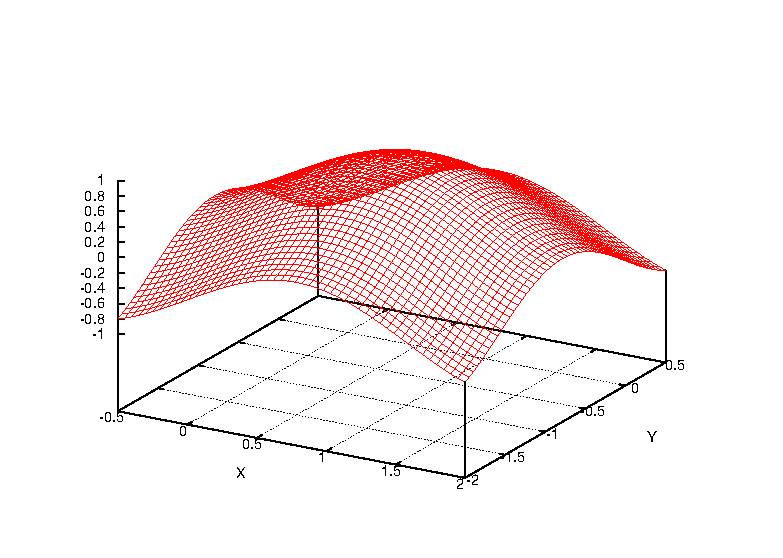
\includegraphics[scale=0.5]{./images/exact.eps}
  \caption{Exact Solution of Poisson's Equation}
  \label{fig:exactPoiss}
\end{figure}

Two simulation runs were performed -- one in serial mode and the other
one in parallel mode using the Message Passing Interface (MPI) with 16
configured nodes. Both runs are configured with $\delta=0.01$ which
yields 251 grid points. \prettyref{fig:approxPoiss} presents both
graphs with the gradient on the surface illustrating the error
(\prettyref{eq:error}) in the conjugate gradient method compared to
the analytical solution (\prettyref{eq:boundaryCond}).

\begin{equation}
  \label{eq:error}
  \epsilon=|u(x,y)-v_{i,j}|
\end{equation}

\begin{figure}[htb]
  \psfrag{X}[B][B][1][0]{x}
  \psfrag{Y}[B][B][1][0]{y}
  \psfrag{ERR}[B][B][1][270]{$\epsilon$}
  \psfrag{PARALLEL}[B][B][1][0]{Parallel}
  \psfrag{SERIAL}[B][B][1][0]{Serial}
  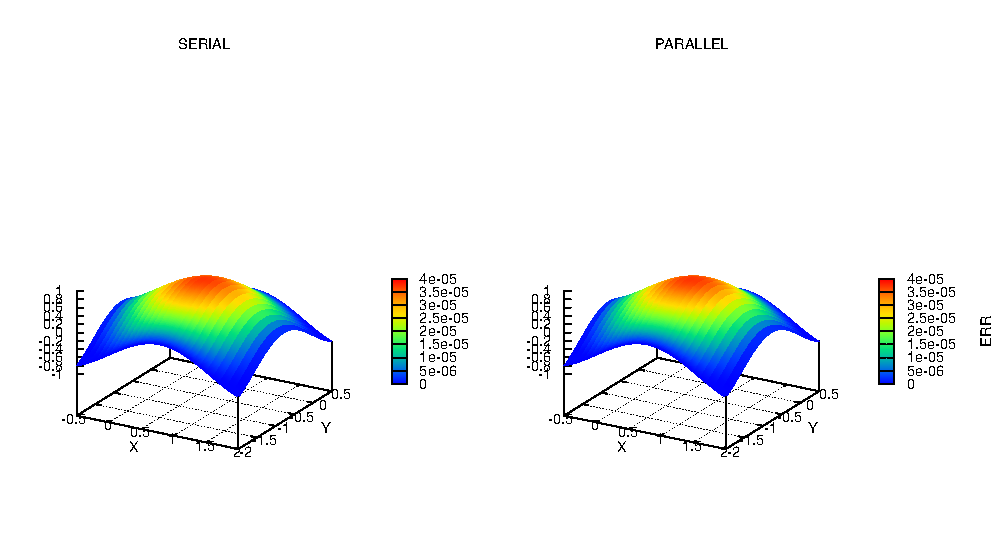
\includegraphics{./images/poiss.eps}
  \caption{Approximate Solution of Poisson's Equation
    $\bigtriangledown^{2}u=-f$}
  \label{fig:approxPoiss}
\end{figure}

\end{document}

%%% Local Variables:
%%% mode: latex
%%% TeX-master: t
%%% End:
